\appendix

\section{Appendix}

The experiments are all run in the same hardware: Intel 14900K CPU (24 cores, 32 threads) for dataset generation, batching and evaluation, and a single NVIDIA RTX 4090 24GB GPU for training.

Runtime may be affected by other processes running on the machine, since it was my everyday computer. They are listed here for reference. \\

Tournaments are held with 100ms per move, and the opening book used is \path{UHO_Lichess_4852_v1.epd}. Each network plays \textbf{at least} 10000 games. Ratings are computed using Ordo, relative to the average (rating=0 is the average) or to the best network (rating=0 is the best network), depending on the experiment. \\

\subsection{Baseline}
\label{appendix:baseline}

\begin{table}[H]
\caption{Network architecture sweep results (L1 $\times$ L2)}
\centering
\begin{adjustbox}{center}

\begin{tabular}{@{} cccccccccc @{}} \toprule
\multirow{2}{*}{\bf Feature set} &
\multicolumn{3}{c}{\bf Train hyperparams} &
\multicolumn{2}{c@{}}{\bf Network} &
\multirow{2}{*}{\makecell{\bf Val loss\\\textit{min}}} &\multirow{2}{*}{\makecell{\bf Rating\\\textit{elo (avg=0)}}} &\multirow{2}{*}{\makecell{\bf Puzzles\\\textit{move acc.}}} &
\multirow{2}{*}{\makecell{\bf Runtime\\\textit{hh:mm:ss}}} \\
\cmidrule(lr){2-4} \cmidrule(l){5-6}
& \bf Batch & \bf LR & \bf Gamma & \bf L1 & \bf L2 & \\
\midrule
    \featureset{HV} & 16384 & 5e-04 & 0.99 & 256 & 32 & 0.00351 & 89.8 $\pm$ 7.3 & \textbf{0.9047} & 1:53:59 \\
\featureset{HV} & 16384 & 5e-04 & 0.99 & 256 & 64 & 0.00342 & 16.5 $\pm$ 7.4 & 0.8976 & 1:54:56 \\
\featureset{HV} & 16384 & 5e-04 & 0.99 & 256 & 128 & 0.00330 & -42.8 $\pm$ 7.6 & 0.8885 & 1:52:29 \\
\featureset{HV} & 16384 & 5e-04 & 0.99 & 256 & 256 & 0.00319 & -65.5 $\pm$ 7.5 & 0.8826 & 2:29:26 \\
\featureset{HV} & 16384 & 5e-04 & 0.99 & 512 & 32 & 0.00309 & 106.6 $\pm$ 7.4 & 0.9027 & 1:54:28 \\
\featureset{HV} & 16384 & 5e-04 & 0.99 & 512 & 64 & 0.00300 & 50.7 $\pm$ 8.2 & 0.8975 & 1:53:44 \\
\featureset{HV} & 16384 & 5e-04 & 0.99 & 512 & 128 & 0.00290 & 12.4 $\pm$ 7.0 & 0.8880 & 1:51:06 \\
\featureset{HV} & 16384 & 5e-04 & 0.99 & 512 & 256 & 0.00279 & -68.9 $\pm$ 8.6 & 0.8790 & 1:51:17 \\
\featureset{HV} & 16384 & 5e-04 & 0.99 & 1024 & 32 & 0.00268 & \textbf{115.1 $\pm$ 8.6} & 0.9032 & 2:15:18 \\
\featureset{HV} & 16384 & 5e-04 & 0.99 & 1024 & 64 & 0.00265 & 52.5 $\pm$ 7.7 & 0.8955 & 2:03:41 \\
\featureset{HV} & 16384 & 5e-04 & 0.99 & 1024 & 128 & 0.00257 & -19.5 $\pm$ 8.6 & 0.8852 & 2:06:39 \\
\featureset{HV} & 16384 & 5e-04 & 0.99 & 1024 & 256 & 0.00246 & -112.1 $\pm$ 8.6 & 0.8725 & 2:32:47 \\
\featureset{HV} & 16384 & 5e-04 & 0.99 & 2048 & 32 & 0.00241 & 102.1 $\pm$ 9.1 & 0.8968 & 3:11:56 \\
\featureset{HV} & 16384 & 5e-04 & 0.99 & 2048 & 64 & 0.00238 & 29.3 $\pm$ 7.2 & 0.8876 & 3:12:46 \\
\featureset{HV} & 16384 & 5e-04 & 0.99 & 2048 & 128 & 0.00234 & -77.5 $\pm$ 7.1 & 0.8779 & 3:29:07 \\
\featureset{HV} & 16384 & 5e-04 & 0.99 & 2048 & 256 & \textbf{0.00221} & -188.8 $\pm$ 8.2 & 0.8678 & 3:27:47 \\
\bottomrule \end{tabular}

\end{adjustbox}
\end{table}

\begin{figure}[H]
\centering
\makebox[\textwidth]{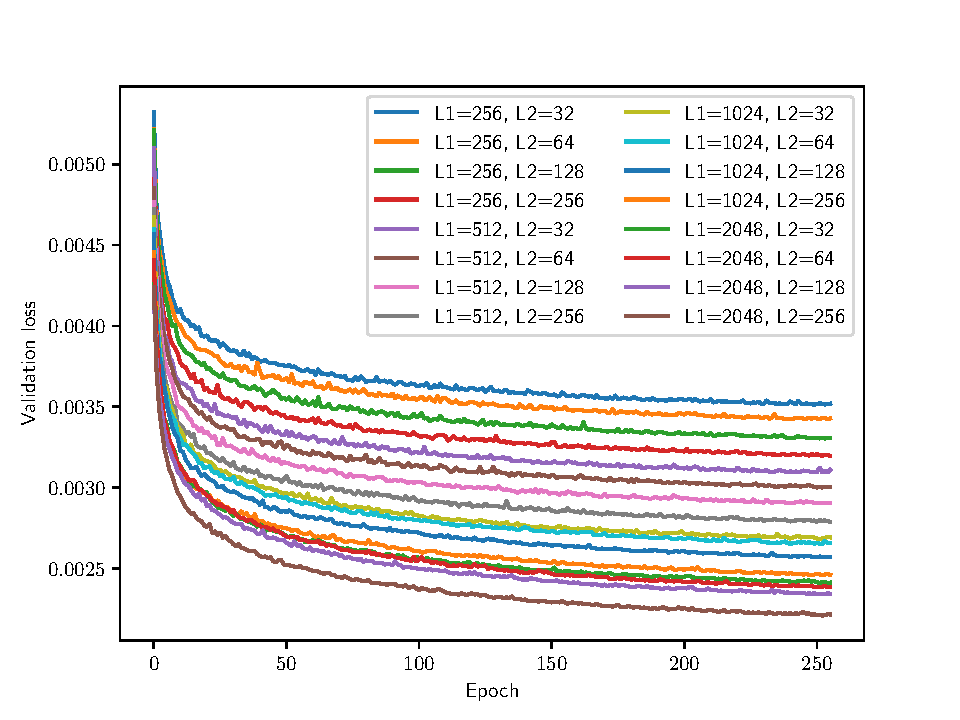
\includegraphics[width=\textwidth]{./dynamic/output/baseline_val_loss.pdf}}
\caption{Network architecture sweep validation loss over epochs (baseline)}
\end{figure}

%%%%%%%%%%%%%%%%%%%%%%%%%%%%%%%%%%%%%%%%%%%%%%%%%%%%%%%%%%%%%%%%%%%
%%%%%%%%%%%%%%%%%%%%%%%%%%%%%%%%%%%%%%%%%%%%%%%%%%%%%%%%%%%%%%%%%%%
%%%%%%%%%%%%%%%%%%%%%%%%%%%%%%%%%%%%%%%%%%%%%%%%%%%%%%%%%%%%%%%%%%%
%%%%%%%%%%%%%%%%%%%%%%%%%%%%%%%%%%%%%%%%%%%%%%%%%%%%%%%%%%%%%%%%%%%
%%%%%%%%%%%%%%%%%%%%%%%%%%%%%%%%%%%%%%%%%%%%%%%%%%%%%%%%%%%%%%%%%%%
%%%%%%%%%%%%%%%%%%%%%%%%%%%%%%%%%%%%%%%%%%%%%%%%%%%%%%%%%%%%%%%%%%%
%%%%%%%%%%%%%%%%%%%%%%%%%%%%%%%%%%%%%%%%%%%%%%%%%%%%%%%%%%%%%%%%%%%

\newpage
\subsection{Axis encoding}
\label{appendix:axes}

\subsubsection{Examples}
\label{appendix:axis_samples}

\begin{figure}[H]
\centering
\subfloat[\centering $\white$ White]{{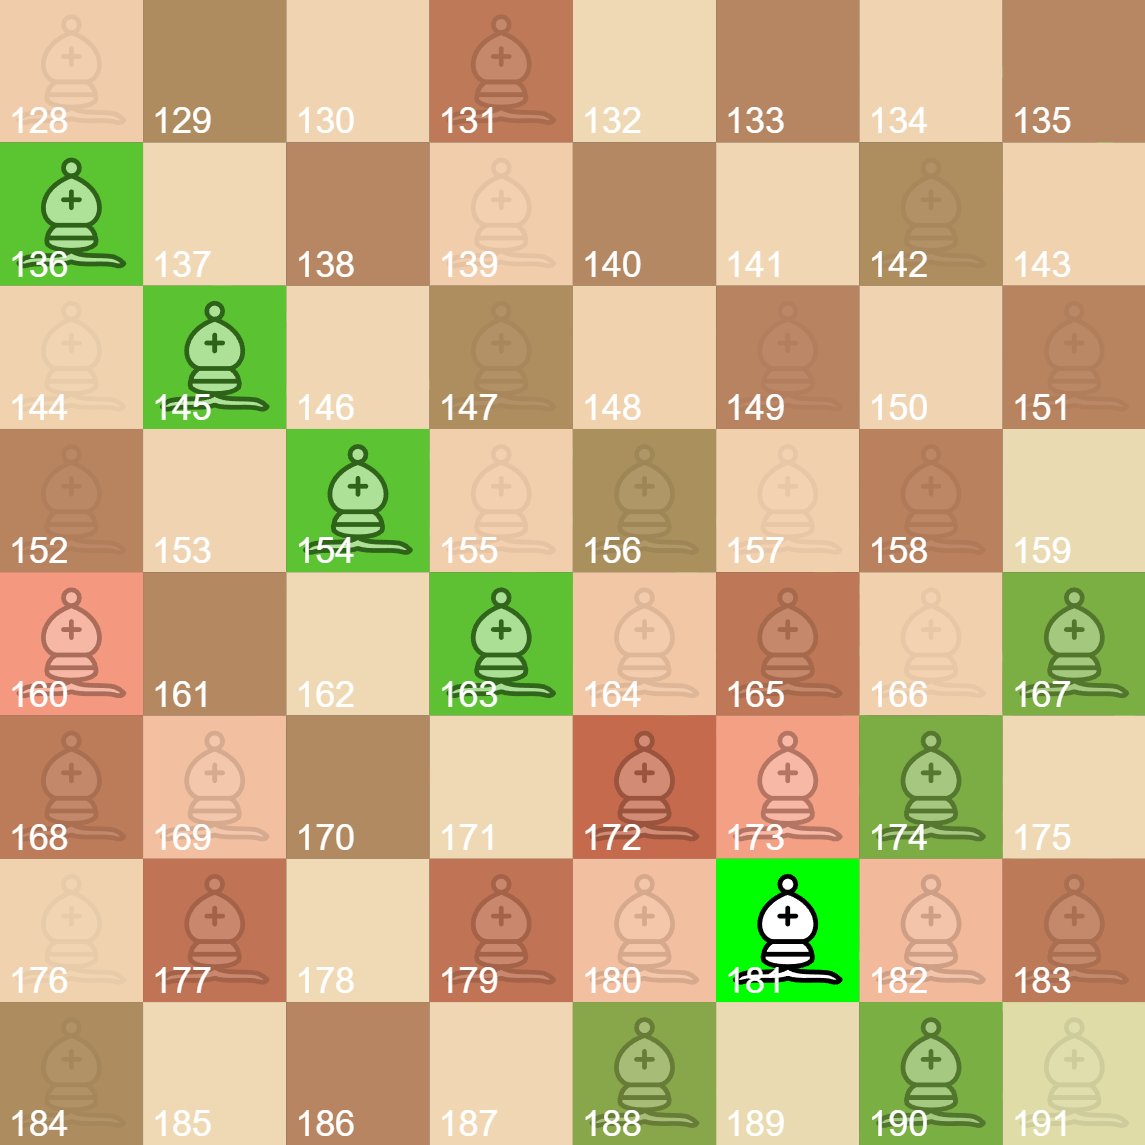
\includegraphics[width=4.65cm]{../assets/results/piece_weights/white_bishop_weights.png} }}
\qquad
\subfloat[\centering $\white$ White]{{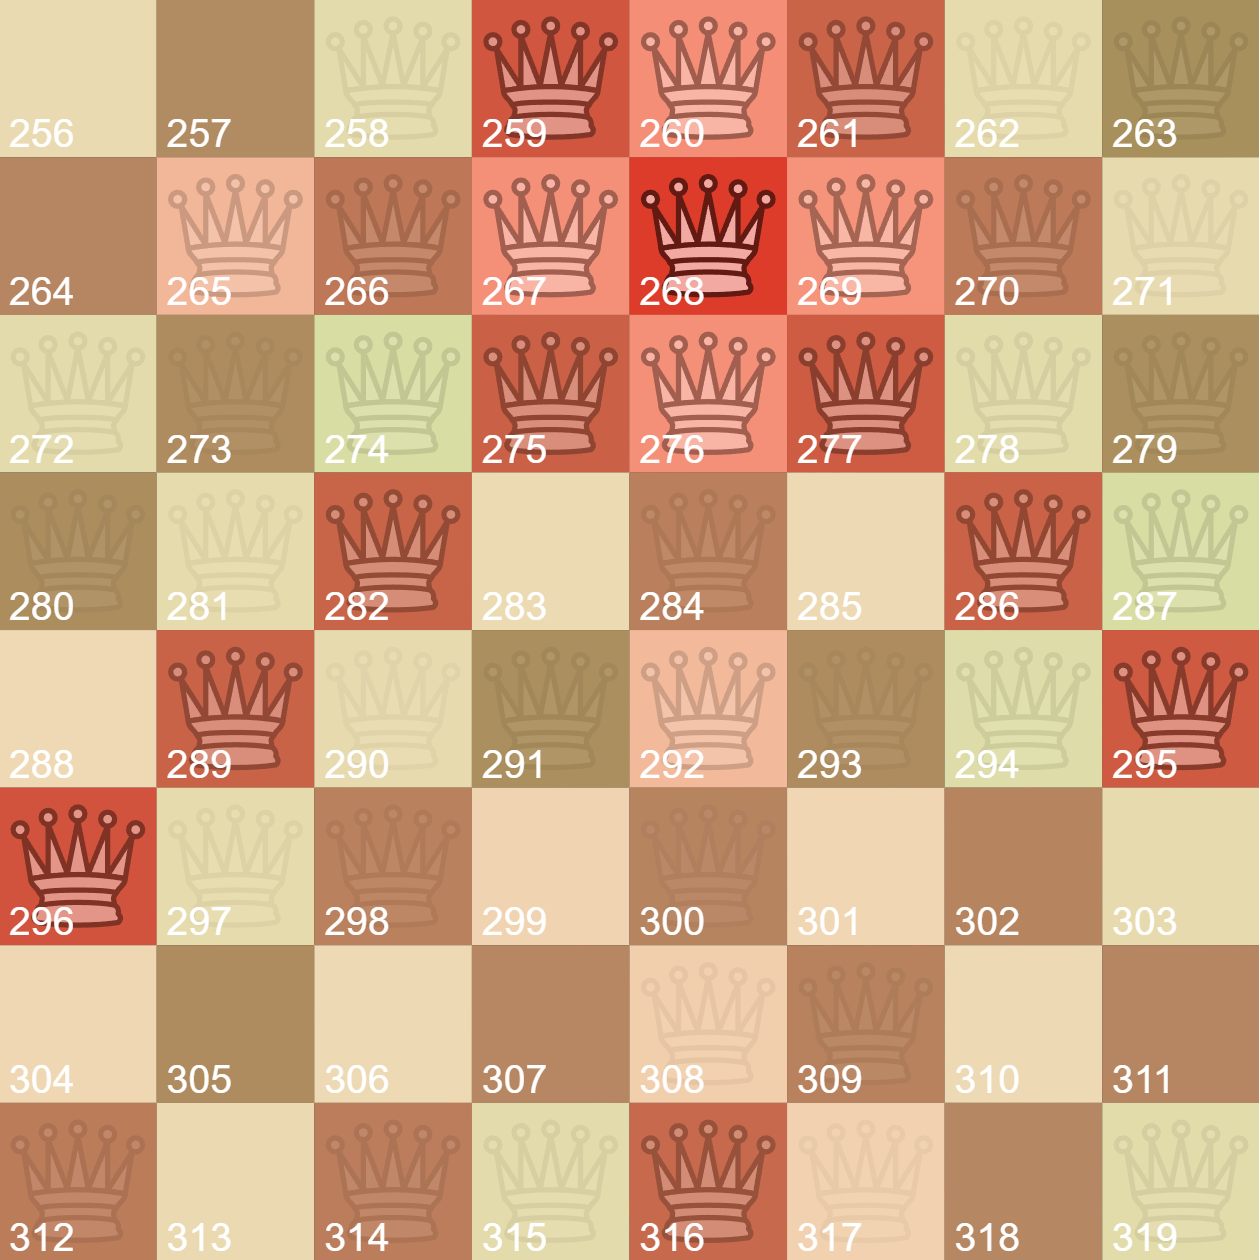
\includegraphics[width=4.65cm]{../assets/results/piece_weights/white_queen_weights.png} }}
\qquad
\subfloat[\centering $\white$ White]{{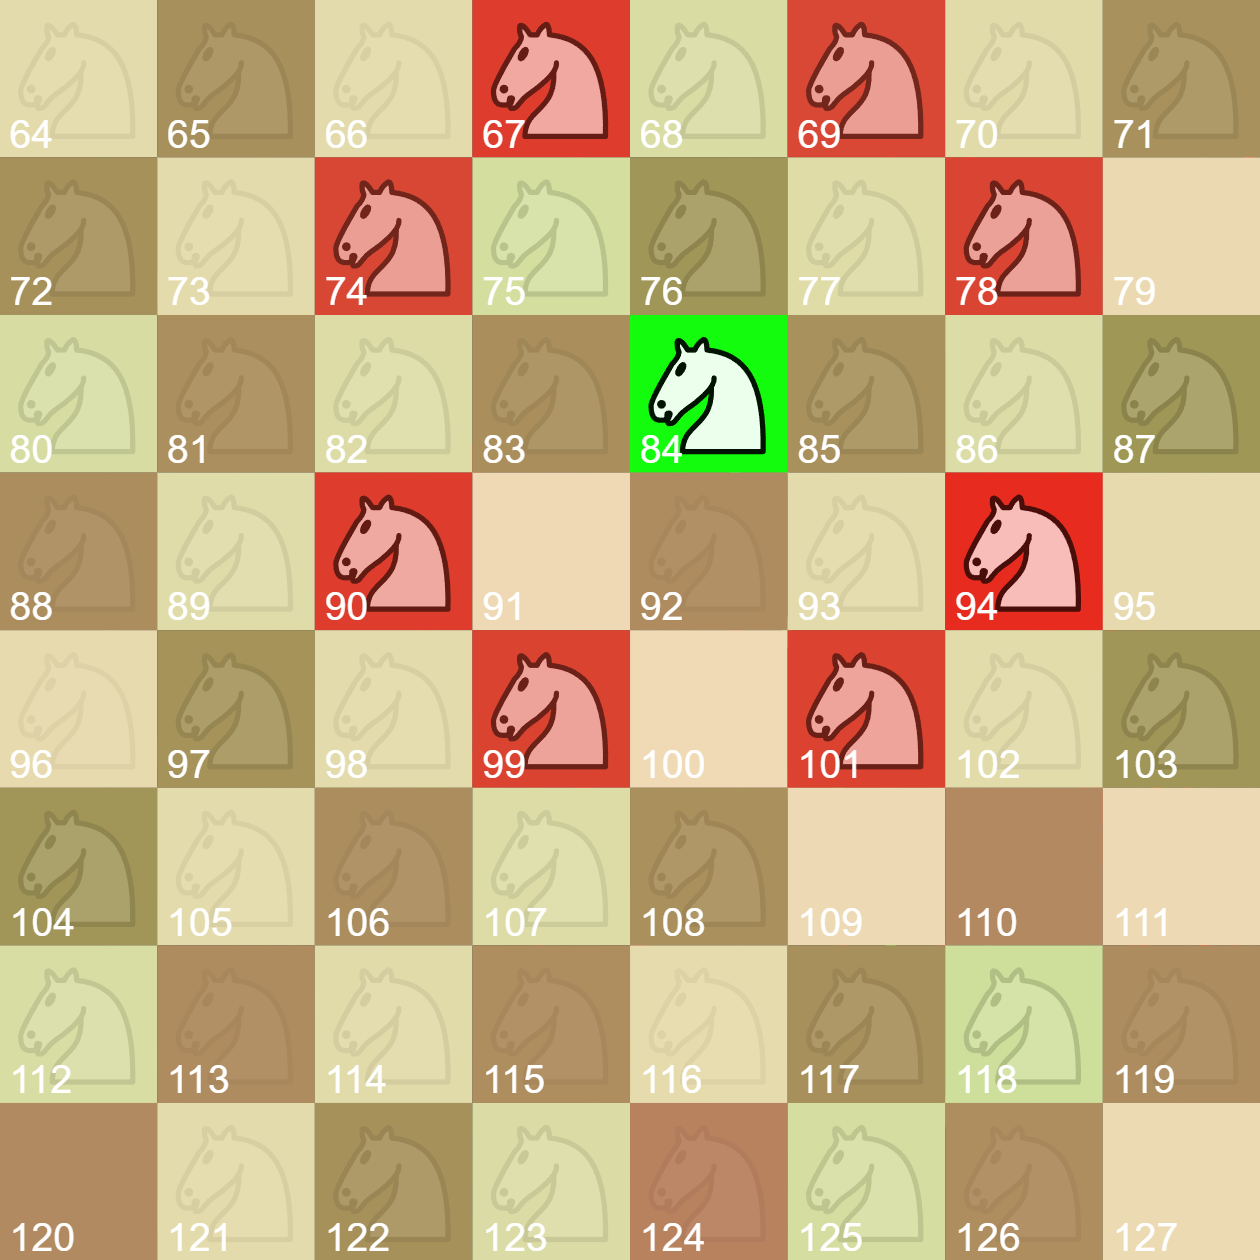
\includegraphics[width=4.65cm]{../assets/results/piece_weights/white_knight_weights.png} }} \\

\subfloat[\centering $\black$ Black]{{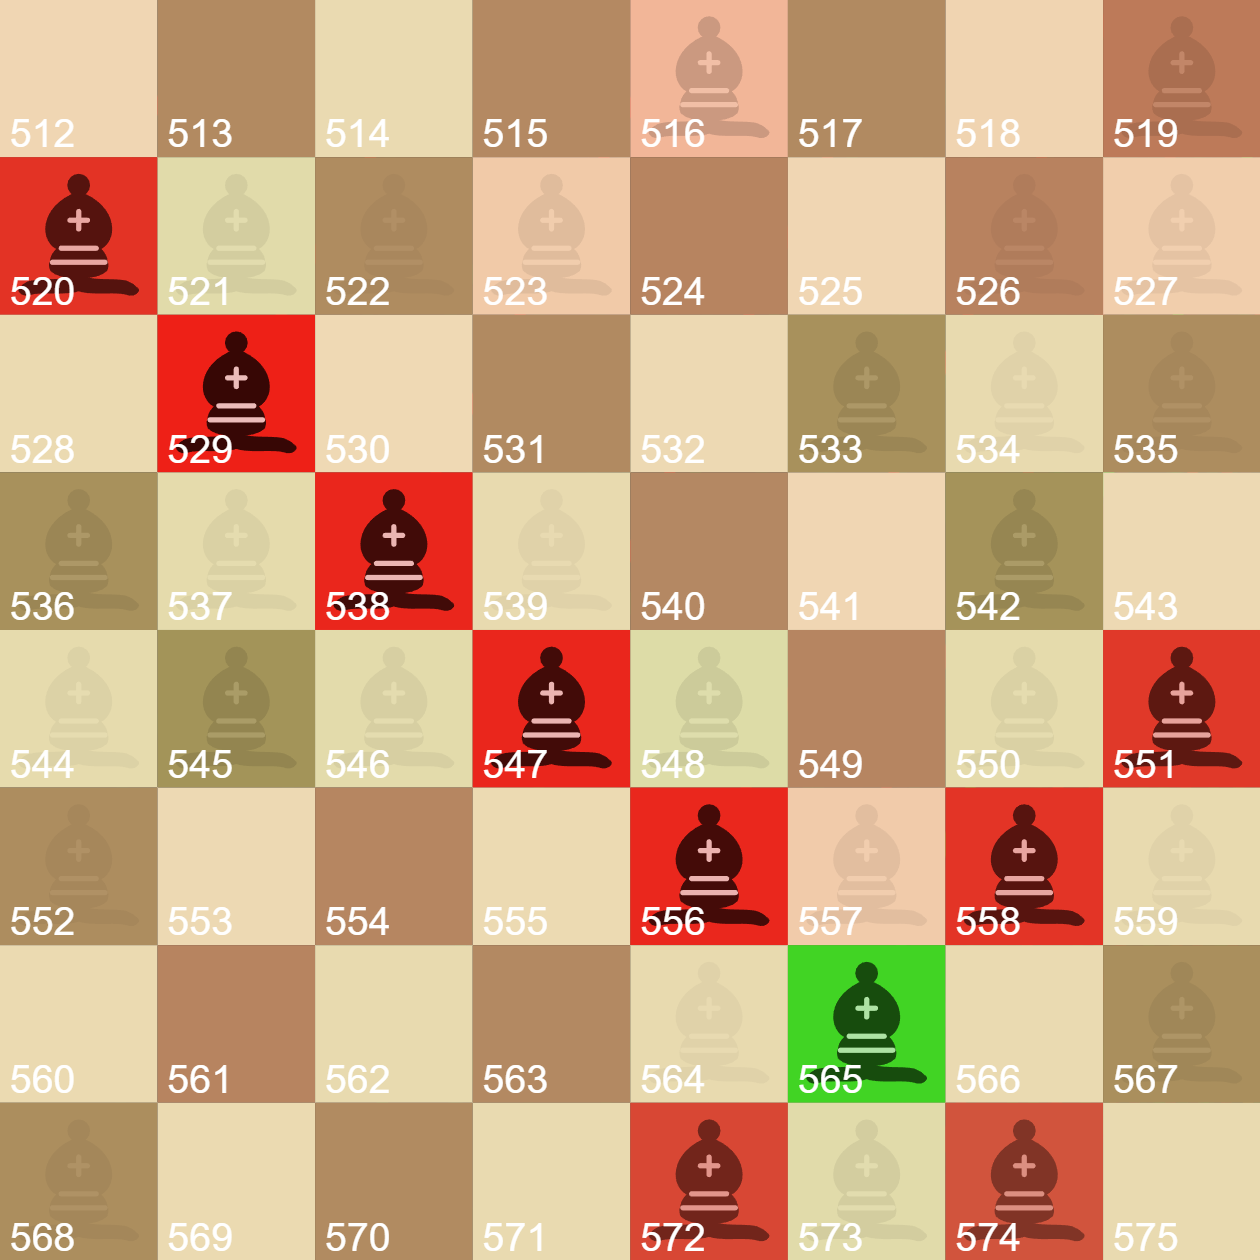
\includegraphics[width=4.65cm]{../assets/results/piece_weights/black_bishop_weights.png} }}
\qquad
\subfloat[\centering $\black$ Black]{{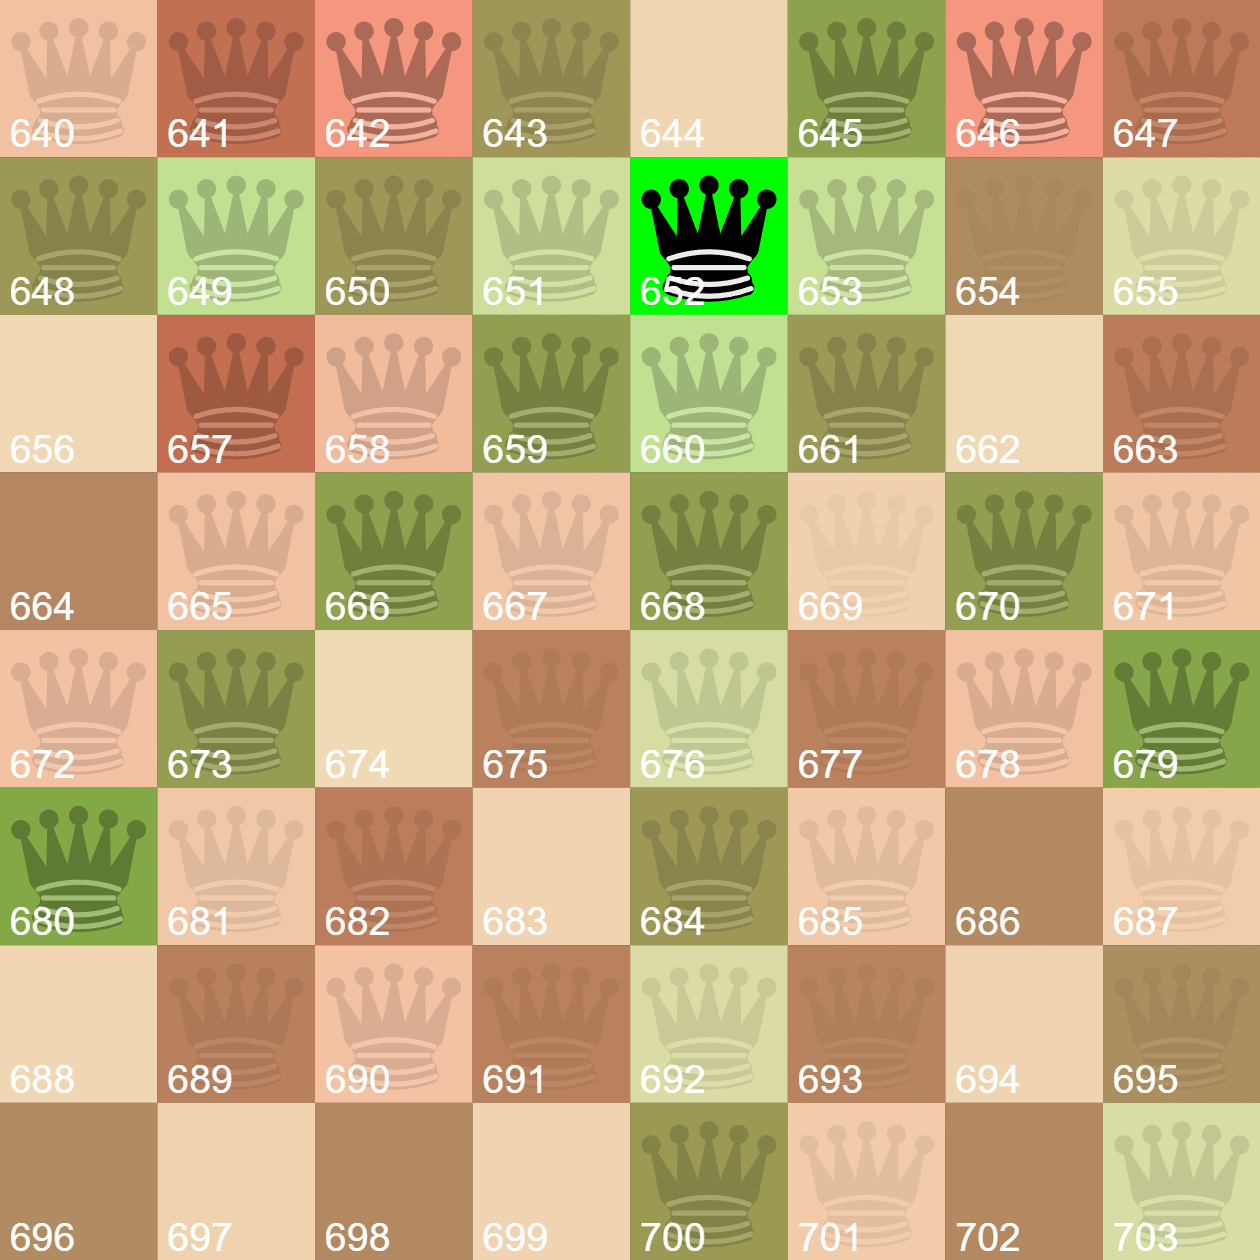
\includegraphics[width=4.65cm]{../assets/results/piece_weights/black_queen_weights.png} }}
\qquad
\subfloat[\centering $\black$ Black]{{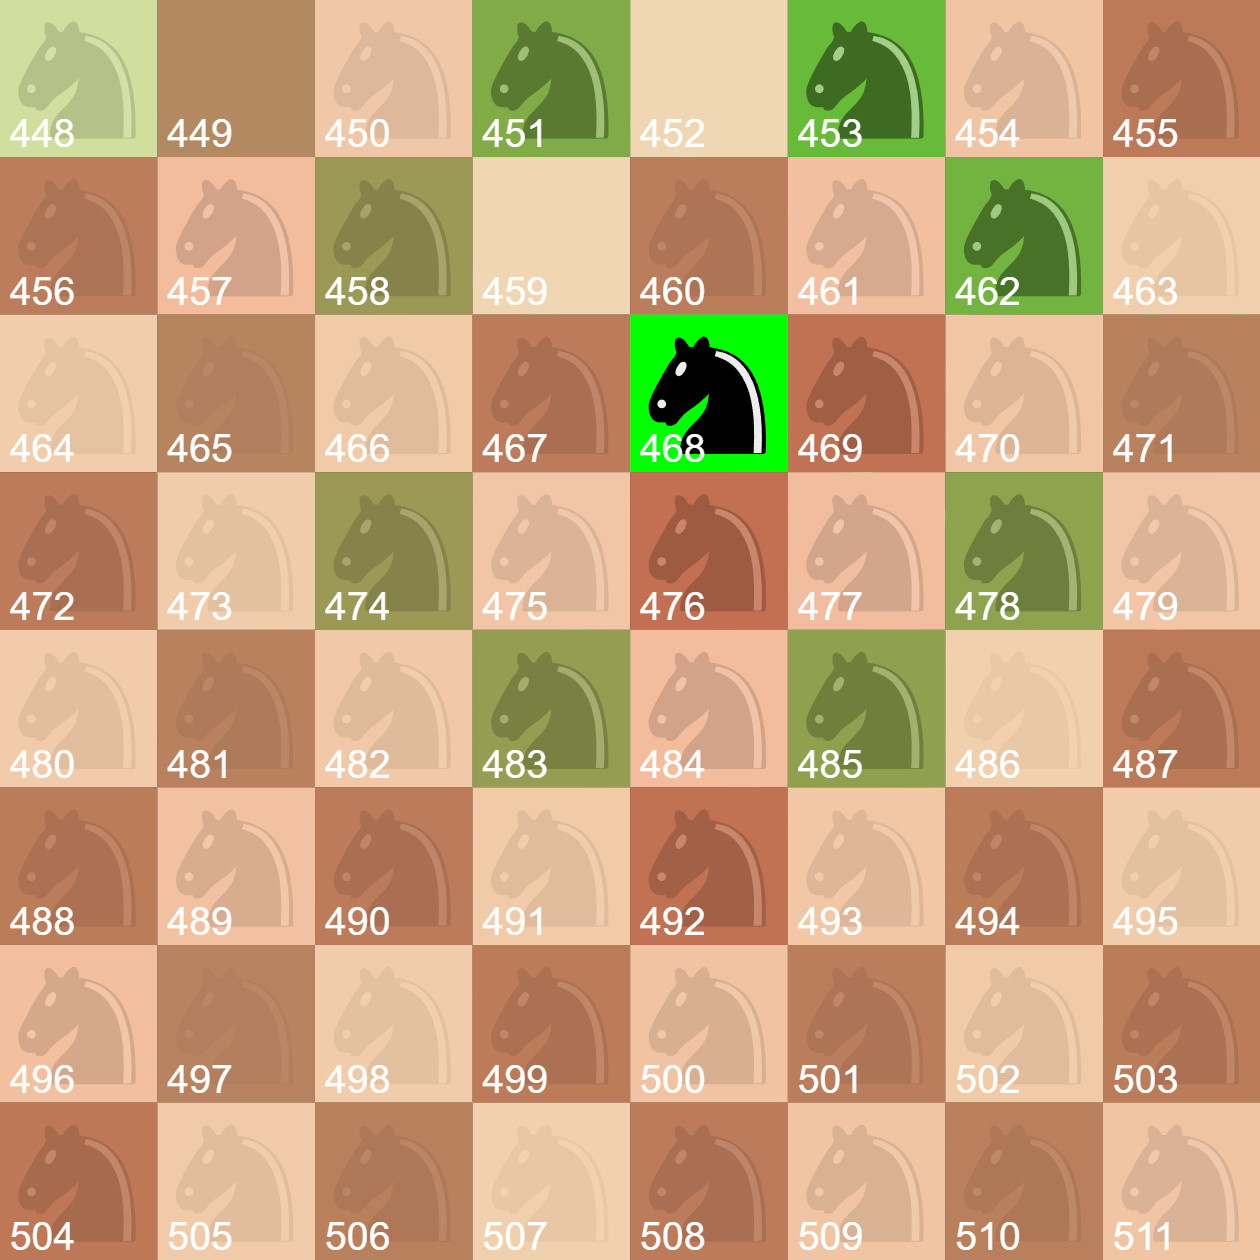
\includegraphics[width=4.65cm]{../assets/results/piece_weights/black_knight_weights.png} }} \\

\caption{Weights of different neurons in the L1 layer, which are connected to features in \featureset{All} with different roles. The intensity represents the weight value, and the color represents the sign. The number is the feature index, specifically \featureset{VH} instead of \featureset{HV} (both are \featureset{All}), because it was prior to the first experiment. Refer to section \ref{sec:axis_encoding}.}
\end{figure}


\subsubsection{Preliminar runs}

    \begin{table}[H]
\caption{Axis feature sets preliminar runs}
\centering
\begin{adjustbox}{center}
\begin{tabular}{@{} cccc|cc @{}}
\toprule
\bf \multirow{2}{*}{Feature set} & \bf \multirow{2}{*}{Run} & \bf Val. loss & \bf Runtime & \bf Rating @ 192 & \bf Rating @ 256 \\
 &  & \textit{min} & \textit{hh:mm:ss} & \textit{TC=100ms/m} & \textit{TC=100ms/m} \\
\midrule
    \multirow{4}{*}{\featureset{D1} + \featureset{D2}} & 1 & \bf0.006707 & 1:44:25 & 2.1 $\pm$ 4.3 & \bf13.5 $\pm$ 4.6\\
 & 2 & 0.006716 & 1:45:46 & -3.9 $\pm$ 5.1 & -0.5 $\pm$ 5.0\\
 & 3 & 0.006729 & 1:47:58 & -4.7 $\pm$ 4.8 & -1.6 $\pm$ 5.3\\
 & 4 & 0.006721 & 1:51:24 & -0.9 $\pm$ 5.3 & -4.0 $\pm$ 5.0\\
\midrule
\multirow{4}{*}{\featureset{H} + \featureset{V}} & 1 & \bf0.005810 & 1:42:35 & -8.6 $\pm$ 5.2 & \bf9.5 $\pm$ 5.5\\
 & 2 & 0.005827 & 1:42:29 & -2.6 $\pm$ 5.4 & -6.5 $\pm$ 5.1\\
 & 3 & 0.005816 & 1:42:59 & 4.8 $\pm$ 4.8 & 2.4 $\pm$ 5.4\\
 & 4 & 0.005825 & 1:43:13 & -6.3 $\pm$ 4.9 & 7.4 $\pm$ 5.2\\
\midrule
\multirow{4}{*}{\featureset{H} + \featureset{V} + \featureset{D1} + \featureset{D2}} & 1 & \bf0.003885 & 2:26:05 & -14.3 $\pm$ 4.9 & -18.1 $\pm$ 4.3\\
 & 2 & 0.003907 & 2:27:30 & 7.2 $\pm$ 5.0 & \bf15.4 $\pm$ 4.7\\
 & 3 & 0.003905 & 2:27:35 & 0.1 $\pm$ 5.3 & 5.2 $\pm$ 4.4\\
 & 4 & 0.003906 & 2:45:19 & 5.7 $\pm$ 5.0 & -1.2 $\pm$ 4.5\\
\midrule
\multirow{4}{*}{\featureset{All}} & 1 & \bf0.003121 & 1:30:34 & -2.9 $\pm$ 4.7 & 4.6 $\pm$ 4.4\\
 & 2 & 0.003129 & 1:30:13 & -4.2 $\pm$ 5.0 & 10.1 $\pm$ 5.4\\
 & 3 & 0.003134 & 1:30:14 & -10.0 $\pm$ 5.2 & \bf10.4 $\pm$ 5.1\\
 & 4 & 0.003147 & 1:30:18 & -9.6 $\pm$ 5.0 & 1.6 $\pm$ 4.8\\
\midrule
\multirow{4}{*}{\featureset{All} + \featureset{D1} + \featureset{D2}} & 1 & 0.003093 & 2:06:54 & -5.0 $\pm$ 4.4 & 1.7 $\pm$ 4.5\\
 & 2 & \bf0.003087 & 2:12:30 & 8.6 $\pm$ 4.3 & \bf12.0 $\pm$ 4.7\\
 & 3 & \bf0.003087 & 2:26:29 & -3.1 $\pm$ 4.9 & 7.9 $\pm$ 3.9\\
 & 4 & 0.003095 & 2:38:25 & -6.1 $\pm$ 4.5 & -16.0 $\pm$ 4.4\\
\midrule
\multirow{4}{*}{\featureset{All} + \featureset{H} + \featureset{V}} & 1 & 0.003086 & 2:05:02 & 1.0 $\pm$ 4.8 & 9.0 $\pm$ 6.0\\
 & 2 & 0.003082 & 2:06:16 & \bf12.9 $\pm$ 4.8 & 7.1 $\pm$ 5.5\\
 & 3 & \bf0.003079 & 2:04:53 & -14.6 $\pm$ 5.1 & 2.3 $\pm$ 5.5\\
 & 4 & 0.003085 & 2:07:18 & -10.1 $\pm$ 4.9 & -7.6 $\pm$ 4.4\\
\midrule
\multirow{4}{*}{\featureset{All} + \featureset{H} + \featureset{V} + \featureset{D1} + \featureset{D2}} & 1 & 0.003071 & 2:49:23 & -18.7 $\pm$ 4.9 & 4.3 $\pm$ 4.6\\
 & 2 & 0.003052 & 2:42:18 & -6.6 $\pm$ 4.6 & -0.6 $\pm$ 4.8\\
 & 3 & 0.003067 & 2:44:26 & 6.5 $\pm$ 4.8 & \bf9.5 $\pm$ 4.6\\
 & 4 & \bf0.003050 & 2:44:34 & -2.9 $\pm$ 5.4 & 8.5 $\pm$ 4.6\\
\toprule
\multicolumn{6}{c}{\makecell{\textbf{Batch size}: 16384, \textbf{LR}: 5e-04, \textbf{Gamma}: 0.99, \textbf{L1}: 512, \textbf{L2}: 32}} \\
\end{tabular}
\end{adjustbox}
\end{table}


\subsubsection{Final results}

    \begin{table}[H]
\caption{Axes feature sets final results}
\centering
\begin{adjustbox}{center}
\begin{tabular}{@{} cccc|cc @{}}
\toprule
\bf \multirow{2}{*}{Feature set} & \bf \multirow{2}{*}{Run} & \bf Val. loss & \bf Runtime & \bf Rating @ 192 & \bf Rating @ 256 \\
 &  & \textit{min} & \textit{hh:mm:ss} & \textit{TC=100ms/m} & \textit{TC=100ms/m} \\
\midrule
    \midrule
\multicolumn{6}{c}{\makecell{None}} \\
\end{tabular}
\end{adjustbox}
\end{table}




%%%%%%%%%%%%%%%%%%%%%%%%%%%%%%%%%%%%%%%%%%%%%%%%%%%%%%%%%%%%%%%%%%%
%%%%%%%%%%%%%%%%%%%%%%%%%%%%%%%%%%%%%%%%%%%%%%%%%%%%%%%%%%%%%%%%%%%
%%%%%%%%%%%%%%%%%%%%%%%%%%%%%%%%%%%%%%%%%%%%%%%%%%%%%%%%%%%%%%%%%%%
%%%%%%%%%%%%%%%%%%%%%%%%%%%%%%%%%%%%%%%%%%%%%%%%%%%%%%%%%%%%%%%%%%%
%%%%%%%%%%%%%%%%%%%%%%%%%%%%%%%%%%%%%%%%%%%%%%%%%%%%%%%%%%%%%%%%%%%
%%%%%%%%%%%%%%%%%%%%%%%%%%%%%%%%%%%%%%%%%%%%%%%%%%%%%%%%%%%%%%%%%%%
%%%%%%%%%%%%%%%%%%%%%%%%%%%%%%%%%%%%%%%%%%%%%%%%%%%%%%%%%%%%%%%%%%%

\newpage
\subsection{Pairwise axes runs}
\label{appendix:pairwise}

\subsubsection{Preliminar runs}

    \begin{table}[H]
\caption{Pairwise feature sets preliminar runs}
\centering
\begin{adjustbox}{center}
\begin{tabular}{@{} cccc|cc @{}}
\toprule
\bf \multirow{2}{*}{Feature set} & \bf \multirow{2}{*}{Run} & \bf Val. loss & \bf Runtime & \bf Rating @ 192 & \bf Rating @ 256 \\
 &  & \textit{min} & \textit{hh:mm:ss} & \textit{TC=100ms/m} & \textit{TC=100ms/m} \\
\midrule
    \multirow{4}{*}{\featureset{All} + \featureset{PH}} & 1 & 0.002954 & 1:56:52 & -2.9 $\pm$ 4.5 & 3.8 $\pm$ 4.0\\
 & 2 & 0.002969 & 1:56:24 & 1.7 $\pm$ 4.7 & 3.3 $\pm$ 4.7\\
 & 3 & 0.002953 & 1:56:12 & -8.7 $\pm$ 4.9 & -1.4 $\pm$ 4.4\\
 & 4 & \bf0.002946 & 1:56:33 & -8.8 $\pm$ 4.7 & \bf13.0 $\pm$ 4.7\\
\midrule
\multirow{4}{*}{\featureset{All} + \featureset{PH} + \featureset{PH}} & 1 & \bf0.002860 & 3:08:28 & -17.9 $\pm$ 5.4 & -5.4 $\pm$ 4.9\\
 & 2 & 0.002865 & 4:10:56 & 1.7 $\pm$ 5.6 & 7.8 $\pm$ 5.5\\
 & 3 & 0.002873 & 3:41:16 & -5.3 $\pm$ 5.0 & 6.2 $\pm$ 5.1\\
 & 4 & 0.002868 & 3:41:38 & 0.8 $\pm$ 5.3 & \bf12.0 $\pm$ 4.9\\
\midrule
\multirow{4}{*}{\featureset{All} + \featureset{PH}} & 1 & \bf0.003022 & 1:57:13 & 2.4 $\pm$ 4.4 & 6.7 $\pm$ 4.6\\
 & 2 & 0.003023 & 2:31:41 & -5.5 $\pm$ 4.6 & 1.8 $\pm$ 4.4\\
 & 3 & 0.003053 & 2:42:28 & -21.7 $\pm$ 4.7 & 0.8 $\pm$ 4.2\\
 & 4 & 0.003033 & 2:44:46 & 7.5 $\pm$ 4.5 & \bf8.0 $\pm$ 4.5\\
\toprule
\multicolumn{6}{c}{\makecell{\textbf{Batch size}: 16384, \textbf{LR}: 5e-04, \textbf{Gamma}: 0.99, \textbf{L1}: 512, \textbf{L2}: 32}} \\
\end{tabular}
\end{adjustbox}
\end{table}


\subsubsection{Final results}

    \begin{table}[H]
\caption{Pairwise feature sets final results}
\centering
\begin{adjustbox}{center}
\begin{tabular}{@{} cccccc @{}}
\toprule
\bf \multirow{2}{*}{Feature set} & \bf \multirow{2}{*}{Run} & \bf \multirow{2}{*}{Epoch} & \bf Val. loss  & \bf Rating & \bf TBD \\
 &  &  & \textit{min}  & \textit{TC=100ms/m} &  \\
\midrule
    \featureset{All} + \featureset{PH} & 4 & 256 & 0.002946 & \bf-8.4 $\pm$ 5.0\\
\featureset{All} + \featureset{PH} + \featureset{PV} & 4 & 256 & \bf0.002868 & -37.6 $\pm$ 4.9\\
\featureset{All} + \featureset{PV} & 4 & 256 & 0.003033 & -38.2 $\pm$ 4.8\\
\toprule
\multicolumn{6}{c}{\makecell{\textbf{Batch size}: 16384, \textbf{LR}: 5e-04, \textbf{Gamma}: 0.99, \textbf{L1}: 512, \textbf{L2}: 32}} \\
\end{tabular}
\end{adjustbox}
\end{table}



% \begin{table}[H]
% \caption{Pairwise feature sets sweep results\\(Games in tournament $\approx 24000$ each)}
% \centering
% \begin{adjustbox}{center}
% 
\begin{tabular}{@{} ccccccccc @{}} \toprule
\multirow{2}{*}{\bf Feature set} &
\multicolumn{3}{c}{\bf Train hyperparams} &
\multicolumn{2}{c@{}}{\bf Network} &
\multirow{2}{*}{\makecell{\bf Val. loss\\\textit{min}}} &\multirow{2}{*}{\makecell{\bf Rating\\\textit{elo (rel. to \featureset{All})}}} &
\multirow{2}{*}{\makecell{\bf Runtime\\\textit{hh:mm:ss}}} \\
\cmidrule(lr){2-4} \cmidrule(l){5-6}
& \bf Batch & \bf LR & \bf Gamma & \bf L1 & \bf L2 & \\
\midrule
    \featureset{All} + \featureset{PH} & 16384 & 5e-04 & 0.99 & 512 & 32 & 0.00296 & \textbf{-0.5 $\pm$ 5.1} & 2:26:00 \\
\midrule
\featureset{All} + \featureset{PV} & 16384 & 5e-04 & 0.99 & 512 & 32 & 0.00303 & -14.1 $\pm$ 4.5 & 2:20:57 \\
\midrule
\featureset{All} + \featureset{PH} + \featureset{PV} & 16384 & 5e-04 & 0.99 & 512 & 32 & \textbf{0.00287} & -32.8 $\pm$ 4.7 & 3:32:35 \\
\midrule
\featureset{H} + \featureset{V} + \featureset{PH} + \featureset{PV} & 16384 & 5e-04 & 0.99 & 512 & 32 & 0.00421 & nan $\pm$ nan & 2:52:24 \\
\bottomrule \end{tabular}

% \end{adjustbox}
% \end{table}


%%%%%%%%%%%%%%%%%%%%%%%%%%%%%

\newpage
\subsection{\texttt{emitPlainEntry} code}
\label{appendix:emitPlainEntry}

\lstset{
  %backgroundcolor=\color{gray!10},  
  basicstyle=\ttfamily,
  columns=fullflexible,
  breakatwhitespace=false,      
  breaklines=true,                
  captionpos=b,                    
  commentstyle=\color{green}, 
  extendedchars=true,              
  frame=single,                   
  keepspaces=true,             
  keywordstyle=\color{blue},      
  language=c++,                 
  numbers=none,                
  numbersep=5pt,                   
  numberstyle=\tiny\color{blue},
  rulecolor=\color{white},        
  showspaces=false,               
  showtabs=false,                 
  stepnumber=5,                  
  stringstyle=\color{red!60!blue},
  tabsize=3,                      
  title=\lstname                
}
\begin{lstlisting}
void emitPlainEntry(std::string& buffer, const TrainingDataEntry& plain)
{
    buffer += plain.pos.fen();
    buffer += ',';
    buffer += std::to_string(plain.score);
    buffer += ',';
    buffer += chess::uci::moveToUci(plain.pos, plain.move);
    buffer += '\n';
}
\end{lstlisting}

